%!TEX TS-program = make
% This is "sig-alternate.tex" V2.0 May 2012
% This file should be compiled with V2.5 of "sig-alternate.cls" May 2012
\documentclass{sig-alternate}
%\documentclass{acm_proc_article-sp}

%\PassOptionsToPackage{pdftex}{graphicx}
\usepackage{graphviz}

\usepackage[numbers,sort]{natbib} % auto-sort citation by number
\usepackage[pdftex]{xcolor}

\usepackage[protrusion=true,expansion=true]{microtype}


\usepackage{syntax}
\grammarparsep 0pt
\grammarindent 8em
%
% TODO items in red
%
\newcommand\todo[1]{\textcolor{red}{#1}}

\begin{document}

%
% --- Author Metadata here ---
%\conferenceinfo{WOODSTOCK}{'97 El Paso, Texas USA}
%\CopyrightYear{20015} % Allows default copyright year (20XX) to be over-ridden - IF NEED BE.
%\crdata{0-12345-67-8/90/01}  % Allows default copyright data (0-89791-88-6/97/05) to be over-ridden - IF NEED BE.
% --- End of Author Metadata ---

\title{The Spack Package Manager:\\
Bringing order to HPC software chaos
\titlenote{\small This work was performed under the auspices of the U.S.
Department of Energy by Lawrence Livermore National Laboratory under Contract DE-AC52-07NA27344.}}
%\subtitle{}
\numberofauthors{7}
\author{
\alignauthor Todd Gamblin\\
       \email{tgamblin@llnl.gov}
\and
\alignauthor Matthew Legendre\\
       \email{legendre1@llnl.gov}
\and
\alignauthor Gregory L. Lee\\
       \email{lee218@llnl.gov}
\and
\alignauthor Adam Moody\\
       \email{moody20@llnl.gov}
\and
\alignauthor Bronis R. de Supinski\\
       \email{bronis@llnl.gov}
\and
\alignauthor Scott Futral\\
       \email{futral@llnl.gov}
\and\\
%
\affaddr{Lawrence Livermore National Laboratory}
%\affaddr{Computation Directorate}\\
%\affaddr{Livermore, CA 94550}
}

\maketitle

\begin{abstract}
	%!TEX root = paper.tex

Large HPC centers spend considerable time supporting software for thousands of users, but the complexity of HPC software is quickly outpacing the capabilities of existing software management tools. Scientific applications require specific versions of compilers, MPI implementations, and dependency libraries, so using a single, standard software stack is infeasible.  However, managing many configurations is difficult because the configuration space is exponential in size.
%
Spack is a package manager used at Lawrence Livermore National Laboratory (LLNL) to manage software complexity. Spack provides a novel, recursive specification syntax to invoke parametric builds of packages and dependencies.  It allows any number of builds to coexist on the same system, and it ensures that installed packages can find their dependencies, {\it regardless of the environment}. We show through real-world use cases that Spack supports a diverse and demanding user base, bringing order to HPC software chaos.

\end{abstract}


% A category with the (minimum) three required fields
%\category{H.4}{Information Systems Applications}{Miscellaneous}
%A category including the fourth, optional field follows...
%\category{D.2.8}{Software Engineering}{Metrics}[complexity measures, performance measures]

%\terms{Theory}

%\keywords{package management, software configuration,
%high performance, parallel, system administration, build systems}

%!TEX root = paper.tex

\section{Introduction}
\label{sec:intro}

\todo{1 page}









\begin{verbatim}
- Why do supercomputing centers need this?

	- specs
		- describe concisely
		- query installed stuff
		- modules require standardized set of names (no order)

	- flexibility (managing combinatoric configuration space)

	- RPATHs instead of (or in addition to) modules
		- pkgs work as built when run
		- spack means there is no module incantation required

	- code teams can build own libs & stacks

	- Contributions:
		1. Flexible mechanism for specifying and querying config space (spec)
		2. Implementation of this in spack
		3. 3 detailed use cases outlining our experiences at LLNL
			a. combinatoric versions
			b. multi-version python installation
			c. site-specific and user-specific policies
\end{verbatim}


%!TEX root = spack-sc15.tex

\section{Common Practice}
\label{sec:motivation}

\paragraph{Meta-build Systems}
{\it Meta-build systems} such as Contractor, WAF, and
MixDown~\cite{amundson:contractor,epperly+:mixdown,epperly+:mixdown-report,nagy:waf} are
related to package managers, but they focus on ensuring that a single
package builds with its dependencies.  MixDown notably provides excellent
features for ensuring consistent compiler flags in a build.
However, these systems do not provide facilities to manage
large package repositories or combinatorial versioning.

\paragraph{Traditional Package Managers}
Package managers automate the installation of complex sets of software packages.
{\it Binary package managers} such as RPM, yum, and APT~\cite{foster+:rpm03,silva:apt01,yum} are integrated with most
OS distributions, and they are used to ensure that dependencies
are installed before packages that require them.
Anaconda~\cite{anaconda,conda}, uses the same approach but
is designed to run on top of a host OS.
These tools largely solve the problem of managing a {\it single} software
stack, which works well for the baseline OS and drivers, which are
common to all applications on a system.
These tools assume that each package has only a single version,
and most install packages in a single, inflexible location.
To install multiple configurations, users must create custom, combinatorial
naming schemes to avoid conflicts. They typically require root
privileges and do not optimize for specific hardware.

{\it Port systems} such as Gentoo, BSD Ports, MacPorts, and
Homebrew~\cite{bsdports,groffen:gentoo-prefix,homebrew,macports,thiruvathukal:gentoo04}
build packages from source instead of installing from a pre-built binary.
Most port systems suffer from
the same versioning and naming issues as traditional package managers.
Some allow multiple versions to be installed in the same
prefix~\cite{groffen:gentoo-prefix}, but again the burden is on package
creators to manage conflicts. This burden effectively restricts installations
to a few configurations.


\paragraph{Virtual Machines and Containers}

Packaging problems arise in HPC because a supercomputer's hardware, OS, and
file system are shared by many users with different requirements.  The classic
solution to this problem is to use virtual
machines (VMs)~\cite{barham2003xen,rosenblum1999vmware,smith2005architecture}
or lightweight virtualization techniques like Linux
containers~\cite{felter2014updated,merkel2014docker}. This model allows each
 user to have a personalized environment with its own package manager, and it
has been very successful for servers at cloud data centers. VMs typically
have near-native compute performance but low-level HPC network drivers still
exhibit major performance issues. VMs are not well supported on many
non-Linux operating systems, an issue for the lightweight
kernels of bleeding-edge Blue Gene/Q and Cray machines.
Finally, each VM still uses a traditional package manager,
so running many configurations still requires a large number of VMs.
For facilities, this profusion of VMs is a security concern because it
complicates mandatory patching. Also, managing  a large number of VM
environments is tedious for users.

\begin{table*}\centering
\begin{tabular}{|l|l|}
\hline
Site           & Naming Convention \\
\hline
\hline
LLNL & {\tt / usr / global / tools / \$arch / \$package / \$version} \\
           & {\tt / usr / local~ / tools / \$package-\$compiler-\$build-\$version } \\
\hline
ORNL~\cite{jones+:cug08}  & {\tt / \$arch / \$package / \$version / \$build} \\
\hline
TACC / Lmod~\cite{mclay:lmod-tutorial}& {\tt / \$compiler-\$comp\_version / \$mpi / \$mpi\_version / \$package / \$version} \\
\hline
\hline
Spack default                  & {\tt / \$arch / \$compiler-\$comp\_version / \$package-\$version-\$options-\$hash} \\
\hline
\end{tabular}
\caption{
	Software organization of various HPC sites.
	\label{tab:naming-conventions}
}
\end{table*}

\paragraph{Manual and Semi-automated Installation}

To cope with software diversity, many HPC sites use a combination of existing
package managers and either manual or semi-automated installation.
For the baseline OS, many sites maintain traditional binary
packages using the vendor's package manager. LLNL maintains a Linux
distribution, CHAOS~\cite{chaos} for this purpose, which is managed using RPM.
The popular ROCKS~\cite{rocks} cluster distribution uses RPM and Anaconda
in a similar fashion.
%
For custom builds, many sites adhere to detailed naming conventions
that encode information in file system paths.
Table~\ref{tab:naming-conventions} shows several sites' conventions.
LLNL uses the APT package manager for installs
in the {\tt /usr/local/tools} file system and {\tt /usr/global/tools}
for manual installs.
Oak Ridge National Laboratory (ORNL) uses hand installs but adheres
to strict scripting conventions
to reproduce each build~\cite{jones+:cug08}.
The Texas Advanced Computing Center (TACC) relies heavily on locally maintained RPMs.

From the conventions in Table~\ref{tab:naming-conventions},
we see that most sites use some combination of architecture, compiler version,
package name, package version, and a custom (up to the author, sometimes
encoded) build identifier.  TACC and many other sites also explicitly
include the MPI version in the path. MPI is explicitly called out
because it is one of the most common software packages for HPC.
However, it is only one of many dependencies that go into a build.
None of these naming conventions covers the entire configuration
space, and none has a way to represent, e.g., two builds that are identical
save for the version of a particular dependency library.  In our experience
at LLNL, naming conventions like these have not succeeded because
users want more configurations than we can represent with a practical
directory hierarchy. Staff frequently install nonconforming packages
in nonstandard locations with ambiguous names.

\paragraph{Environment Modules and RPATHs}\label{sec:env-rpath}

Diverse software versions not only present problems for build and installation;
they also complicate the runtime environment. When launched, an executable
must determine the location of its dependency libraries, or it will not run.
Even worse, it may find the wrong dependencies and subtly produce incorrect results.
Statically linked binaries do not have this issue, but modern
operating systems make extensive use of dynamic linking.
By default, the dynamic loader on most systems is configured to search only
system library paths such as {\tt /lib}, {\tt /usr/lib}, and
{\tt /usr/local/lib}.  If binaries are installed in other locations, the
{\it user} who runs the program must typically add dependency library paths to
{\tt LD\_LIBRARY\_PATH} (or a similar environment variable) so that the loader
can find them.  Often, the user is not the same person who installed the library,
and even advanced users may have difficulty determining which paths to add.

Many HPC sites address this problem using {\it environment modules}, which
allow users to ``load'' and ``unload'' such settings dynamically using simple
commands. Environment modules emerged in 1991, and there are many implementations~\cite{dotkit,furlani+:lisa91,furlani+:lisa96,mclay:lmod,mclay:lmod-tutorial}.
The most advanced of these, Lmod~\cite{mclay:lmod,mclay:lmod-tutorial},
provides software hierarchies that are similar to the naming conventions in
Table~\ref{tab:naming-conventions} and allow users to load a software stack
quickly if they know which one is required.

The alternative to per-user environment settings is to embed library search
paths in installed binaries at compile time. When set this way, the search
path is called an {\tt RPATH}. {\tt RPATHs} and environment modules are not
mutually exclusive. Modules can still be used to set variables that are
unrelated to linking, such as {\tt MANPATH} and {\tt PATH}.  Adding
{\tt RPATHs} still ensures that binaries run correctly,
regardless of whether the right module is loaded. LC installs software with
both {\tt RPATHs} and {\tt dotkit}~\cite{dotkit} modules.

\paragraph{Modern Package Managers}

Recently, a number of HPC package managers have emerged that manage
multi-configuration builds.
%
ORNL uses the Smithy~\cite{digirolamo:smithy} installation tool. It
can generate module files, but it does not provide any
automated dependency management; it only checks whether a package's
prerequisites have already been installed by the user.

The Nix~\cite{dolstra+:icfp08,dolstra+:lisa04} package manager and OS
distribution supports installation of arbitrarily many software
configurations.  As at most HPC sites, it installs each package
in a unique prefix but it does not have a human-readable naming
convention.  Instead, Nix determines the prefix by hashing the package
file and its dependencies.
%% BRONIS: I'm not sure what the following sentence really adds
%%  Nix package files are written in a custom
%% functional language designed for packaging.

The EasyBuild~\cite{hoste+:pyhpc12} tool is in production use at
the University of Ghent and the J\"ulich Supercomputing Center.
It allows multiple versions to be installed at once.  Rather
than setting {\tt RPATHs}, it generates module files
to manage the environment, and it is closely coupled with
Lmod~\cite{geimer+:hust14}.  EasyBuild groups the compiler, MPI, FFT, and
BLAS libraries together in a {\it toolchain} that can be used by
package files. The grouping provides some composability and
separates compiler flags and MPI concerns from client packages.

HashDist~\cite{hashdist} is a meta-build system and package manager
for HPC.  Of the existing solutions, it is the most similar to Spack.
Like Nix, it uses cryptographic versioning and stores installations in
unique directories.
%
Both Nix and HashDist use {\tt RPATHs} in their packages to ensure that
libraries are found correctly at runtime.

\paragraph{Gaps in Current Practice}
The flexible cryptographic versioning of Nix and HashDist manages
the package {\it and} its dependency configuration and can represent any
configuration. However, users cannot easily navigate or query the installed
software.
%The systems are in a sense ``write-only'':
%Nix does not offer a way to view a package's dependencies.
%
EasyBuild and Smithy generate environment modules, which supports some
querying. Naming schemes used in existing module systems, however, cannot
handle combinatorial versions, which the Lmod authors call the
``matrix problem''~\cite{mclay:lmod-tutorial}.

%EasyBuild's attempts to version groups dependencies by adding versions to
%toolchains, but the naming is difficult to understand.
%. Compiler, MPI, and
%some library versions are lumped together, but the results is cryptic, e.g.
%{\tt goolf} stands for ``gcc, openmpi, openblas, ScaLAPACK, FFTW'', and
%its version is meaningless.

%Existing tools do not enforce {\tt RPATHs}, leaving them to package authors.
%This may lead to erroneous runs.

The main limitation of existing tools is the lack of build {\it composability}.
The full set of package versions is combinatorial, and arbitrary combinations
of compiler, MPI version, build options, and dependency versions require
non-trivial modifications to many package files. Indeed, the number of package
files required for most existing systems scales with the number of version
{\it combinations}, not the number of packages, which quickly becomes
unmanageable.  As an example, the EasyBuild system has over 3,300 files for
several permutations of around 600 packages. A slightly different dependency
graph requires an entire new package file hierarchy.  HashDist supports
composition more robustly but does not have first-class parameters for
versions, compilers, or versioned interfaces.
%
HPC sites need better ways to {\it parameterize} packages so that new
builds can be {\it composed} in response to user needs.
%


%!TEX root = spack-sc15.tex

\section{The Spack Package Manager}
\label{sec:implementation}
Based on our experiences at LLNL, we have developed
{\it Spack}, the \underline{S}upercomputing \underline{Pack}age manager.
Spack is written in Python, which we chose for its flexibility
and its increasing use in HPC.
%
Like prior systems, Spack supports an arbitrary number of software
installations, and like Nix it can identify them with hashes.  Unlike any
prior system, Spack provides a language to specify and manage the
combinatorial space of HPC software configurations.

\noindent
Spack provides the following unique features:
\begin{enumerate}
\item Composable packages, explicitly {\bf parameterized} by version, platform,
      compiler, options, and dependencies.
\item A novel, recursive {\bf spec syntax} for dependency graphs and constraints,
      which aids in managing the build parameter space.
\item {\bf Versioned virtual dependencies} to handle versioned, 
      ABI-incompatible interfaces like MPI.
\item A novel {\bf concretization} process that translates an abstract build
      specification into a full, concrete build specification.
\item A build environment that uses {\bf compiler wrappers} to enforce build
      consistency and simplify package writing.
\end{enumerate}

%!TEX root = paper.tex

\subsection{Packages}

%\subsubsection{Package Files}
\begin{figure}
	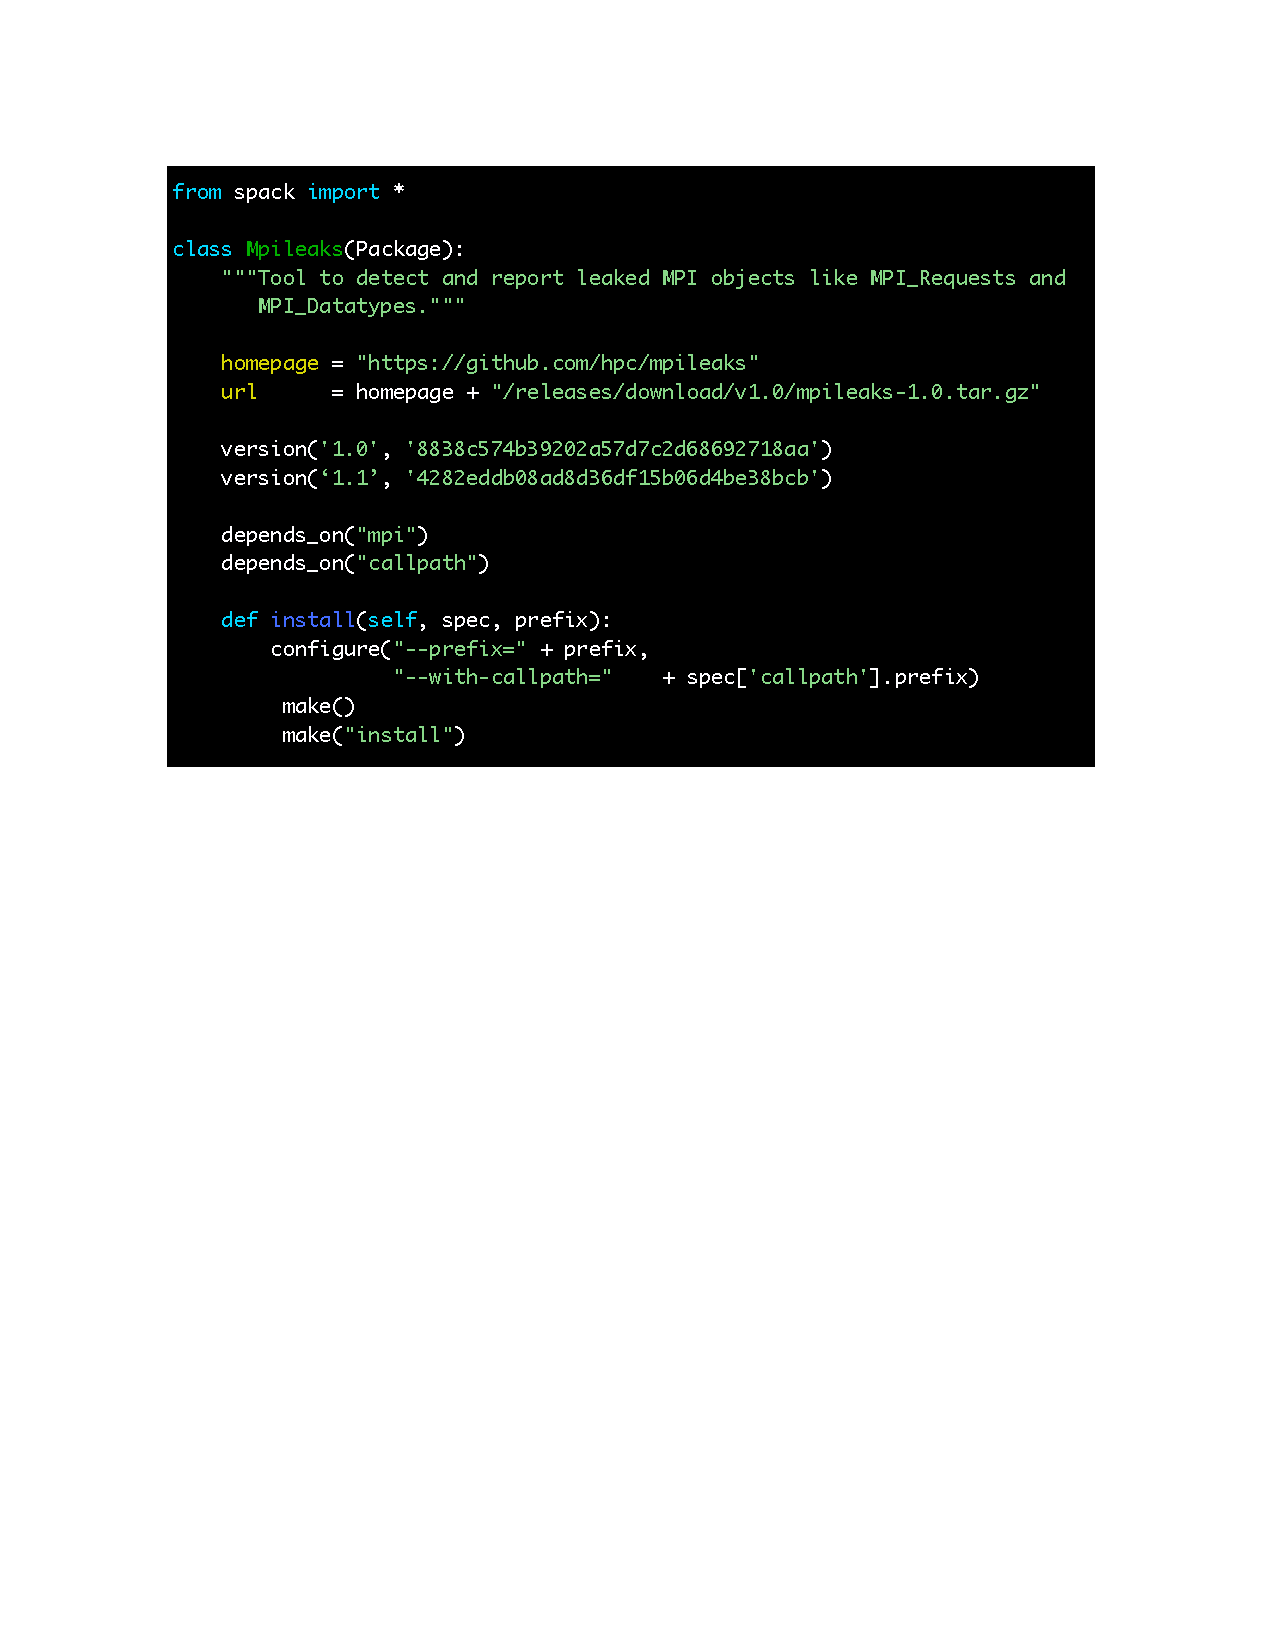
\includegraphics[width=\columnwidth]{code/mpileaks.pdf}
	\caption{
		Spack package for the {\tt mpileaks} tool.
		\label{fig:mpileaks}
	}
\end{figure}

In Spack, packages are build scripts that describe how to build software
artifacts.  Each package is a class written in pure Python to describe
{\it specific} build instructions, and it must extend the {\tt Package}
base class, which implements the more general parts of the build process.
Spack implements a simple, embedded domain-specific language (DSL) to make
packaging easier; it adds special directives such as {\tt depends\_on} and
{\tt version} that add metadata to the class.

Figure~\ref{fig:mpileaks} shows the package for \mpileaks, an LLNL-developed
tool for finding leaks in MPI programs.
Inside the {\tt MpiLeaks} class, the package provides a text description
and a homepage, as well as 
a download URL.  Next, two {\tt version} directives identify known versions
of the package, and MD5 checksums ensure they can be downloaded safely.
Below this, two {\tt depends\_on}
directives indicate prerequisites that must be installed before \mpileaks.
Last, each package defines an {\tt install()} method, which contains the
commands used to build the package.  Spack's DSL allows shell
commands to be invoked as Python functions. Here, the {\tt install()} 
method invokes the familiar {\tt configure}, {\tt make}, and
{\tt make install} build commands, as a shell script would.






%!TEX root = spack-sc15.tex

\begin{figure}
	\begin{subfigure}{\linewidth}
		\centering
		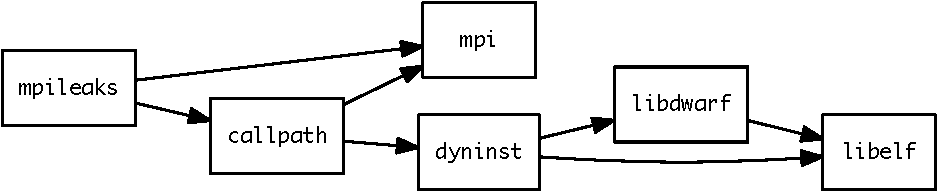
\includegraphics[width=.9\columnwidth]{specs/mpileaks.pdf}
		\caption{
			Spec for {\tt mpileaks}
			\label{fig:specs-mpileaks}
		}
	\end{subfigure}
%
	\begin{subfigure}{\linewidth}
		\centering
		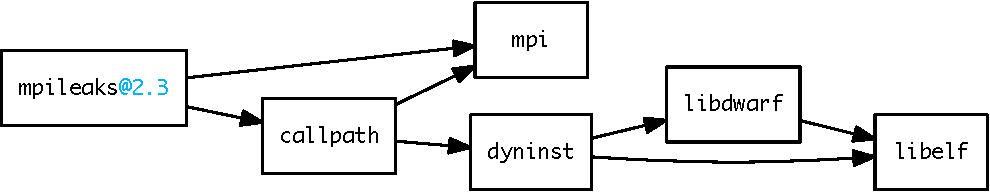
\includegraphics[width=.9\columnwidth]{specs/mpileaks-version}
		\caption{
			{\tt mpileaks@2.3}
			\label{fig:specs-mpileaks-version}
		}
	\end{subfigure}
%
	\begin{subfigure}{\linewidth}
		\centering
		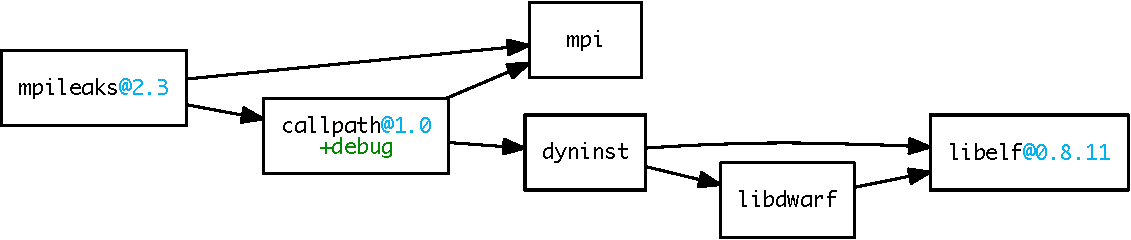
\includegraphics[width=.9\columnwidth]{specs/mpileaks-abstract.pdf}
		\caption{
			{\tt mpileaks@2.3 \^{}callpath@1.0+debug \^{}libelf@0.8.11}
			\label{fig:specs-mpileaks-abstract}
		}
	\end{subfigure}
%
	\caption{
		Constraints applied to {\tt mpileaks} specs.
	}
	\label{fig:specs}
\end{figure}



\subsection{Spack Specs}\label{sec:specs}

Using the simple script in Figure~\ref{fig:mpileaks}, Spack can build many different
versions and configurations of the {\tt mpileaks} package.  In traditional port systems,
package code is structured to build a single version of a package, but in Spack, each
package file is a {\it template} that can be configured and built in many
different ways, according to a set of {\it parameters}.
Spack calls a single build configuration a {\it spec}.
Spack communicates dependencies and parameters to package authors using
the {\tt spec} argument of the {\tt install} method.

\subsubsection{Structure}
To understand specs, consider the {\tt mpileaks} package structure.
Metadata in the {\tt Mpileaks} class (e.g., {\tt version} or
{\tt depends\_on}) describe its relationships with other packages.
The tool has two direct dependencies:
the {\tt callpath} library and {\tt mpi}.  Spack recursively inspects the class definitions
for each dependency and constructs a graph of their relationships.  The result
is a directed, acyclic graph (DAG).\footnote{Spack currently disallows
circular dependencies.}
%
To guarantee a consistent build and to avoid
Application Binary Interface (ABI) incompatibility, we construct
the DAG with only {\it one} version of each package.  Thus, while
Spack can install arbitrarily many configurations of any package,
no two configurations of the same package will ever appear in the same build DAG.

DAGs for {\tt mpileaks} are shown in Figure~\ref{fig:specs}.
Each node represents a package, and each package has five configuration parameters that control
how it will be built: 1) the package version, 2) the compiler with which to
build, 3) the compiler version, 4) named compile-time build options, or
{\it variants}, and 5) the target architecture.


\subsubsection{Configuration Complexity}
A spec DAG has many degrees of freedom, and users cannot reasonably be
expected to understand or to specify all of them.  In our experience at LLNL,
the typical user only cares about a small number of build constraints (if any),
and does not know enough to
specify the rest. For example, a user may know that a certain version of a library like
{\tt boost}~\cite{boost} is required, but only cares that other build parameters are set so that
the build will succeed.
%
Configuration complexity makes the HPC software ecosystem difficult to manage:
too many parameters exist to specify them all. However, the known and
important ones often provide detailed build constraints. Thus, we have two
competing concerns.  We need the ability to specify details
without having to remember all of them.

\subsubsection{Spec Syntax}\label{sec:syntax}
\begin{figure}
{\fontfamily{cmr}\selectfont
\begin{grammar}\small
  <spec>         ::= <id> [ <constraints> ]

  <constraints>   ::= \{ `@' <version-list> | `+' <variant> \newline
                   | `-' <variant> ~~~| `~' <variant> \newline
                   | `\%' <compiler> ~| `=' <architecture> \} \newline
                  [ <dep-list> ]

  <dep-list>  ::= \{ `\textsf \textasciicircum' <spec> \}

  <version-list> ::= <version> [ \{ `,' <version> \} ]

  <version>      ::= <id> | <id> `:' | `:' <id> | <id> `:' <id>

  <compiler>     ::= <id> [ <version-list> ]

  <variant>      ::= <id>

  <architecture> ::= <id>

  <id>           ::= "[A-Za-z0-9_][A-Za-z0-9_.-]*"
\end{grammar}
} % End fontfamily{cmr}
\caption{
	EBNF grammar for spec expressions.
	\label{fig:grammar}
}
\end{figure}


\begin{table*}\centering
\begin{tabular}{|r|p{2.4in}|p{4in}|}
\hline
& {\bf Spec} & {\bf Meaning} \\
\hline
\hline
1&\small\verb|mpileaks|                         & \small {\tt mpileaks} package, no constraints. \\\hline
2&\small\verb|mpileaks@1.1.2|                   & \small {\tt mpileaks} package, version 1.1.2. \\\hline
3&\small\verb|mpileaks@1.1.2 %gcc|              & \small {\tt mpileaks} package, version 1.1.2, built with {\tt gcc} at the default version. \\\hline
4&\small\verb|mpileaks@1.1.2 %intel@14.1 +debug| & \small {\tt mpileaks} package, version 1.1.2, built with Intel compiler version 14.1, \newline with the ``debug'' build option. \\\hline
5&\small\verb|mpileaks@1.1.2 =bgq|              & \small {\tt mpileaks} package, version 1.1.2, built for the Blue Gene/Q platform (BG/Q). \\\hline
6&\small\verb|mpileaks@1.1.2 ^mvapich2@1.9|     & \small {\tt mpileaks} package version 1.1.2, using {\tt mvapich2}  version 1.9 for MPI. \\\hline
7&\small\verb|mpileaks @1.2:1.4 %gcc@4.7.5 -debug =bgq| \newline
      \verb|  ^callpath @1.1 %gcc@4.7.2| \newline
      \verb|  ^openmpi @1.4.7|                & \small%
      {\tt mpileaks} at any version between 1.2 and 1.4 (inclusive), built with gcc 4.7.5,
      without the debug option, for BG/Q, linked with {\tt callpath} version 1.1
      and building {\tt callpath} with {\tt gcc} version 4.7.2, linked with {\tt openmpi} version 1.4.7.    \\
\hline
\end{tabular}
\caption{
	Spack build spec syntax examples and their meaning.
	\label{tab:specs}
}
\end{table*}

We have developed a syntax for specs that allows users to specify
only constraints that matter to them. Our syntax can represent
DAGs concisely enough for command line use.
The spec syntax is recursively defined to allow users to specify
parameters on dependencies as well as on the root of the DAG.
Figure~\ref{fig:grammar} shows the EBNF grammar through which Spack
flexibly supports constraints.

We begin with a simple example.
Consider the case where a user wants to install the {\tt mpileaks} package, but knows
nothing about its structure.  To install the package, the user invokes {\tt spack install}:
%
\begin{minted}[fontsize=\scriptsize]{bash}
    $ spack install mpileaks
\end{minted}
%
Here, {\tt mpileaks} is the simplest possible spec---a single identifier.
Spack converts it into the DAG shown in Figure~\ref{fig:specs-mpileaks}.
Note that even though the spec contains no dependency information, it is still
converted to a full DAG, based on directives supplied in package files. Since
the spec does not constrain the nodes, Spack has leeway when building the
package, and we say that it is {\it unconstrained}.
%
However, a user who wants a specific {\tt mpileaks} version can
request it with a version constraint after the package name:
%
\begin{minted}[fontsize=\scriptsize]{bash}
    $ spack install mpileaks@2.3
\end{minted}
%
Figure~\ref{fig:specs-mpileaks-version} shows that the specific version
constraint is placed on the {\tt mpileaks} node in the DAG, which otherwise
remains unconstrained.
A user who only requires a particular minimum version could use
{\it version range} syntax
and write {\tt @2.3:}.  Likewise, {\tt @2.3:2.5.6} would specify a
version between 2.3 and 2.5.6. In these cases, the user can save time if
Spack already has a version installed that satisfies the spec -- Spack will use
the previously-built installation instead of building a new one.

Figure~\ref{fig:specs-mpileaks-abstract} shows the recursive nature of the spec syntax:
%
\begin{minted}[fontsize=\scriptsize]{bash}
    $ spack install mpileaks@2.3 ^callpath@1.0+debug ^libelf@0.8.11
\end{minted}
%
The caret (\verb|^|) denotes constraints for a particular dependency. The DAG
now has version constraints on {\tt callpath} {\it and} {\tt libelf},
and the user has requested the {\tt debug} variant of the {\tt callpath} library.

Recall that Spack guarantees that only a single version of any package occurs
in a spec.  Within a spec, each dependency can be uniquely
identified by its package name alone.  Therefore, the user does not need to consider
DAG connectivity to add constraints but instead must only know that
{\tt mpileaks} depends on {\tt callpath}.
Thus, dependency constraints can appear in an arbitrary order.

Table~\ref{tab:specs} shows further examples of specs, ranging from
simple to complex. These examples show how Spack's constraint
notation covers the rest of the HPC package parameter space.

{\bf Versions.}
Version constraints are denoted with {\tt @}. Versions
can be precise ({\tt @2.5.1}) or denote a range ({\tt @2.5:4.4}),
which may be open-ended ({\tt @2.5:}).
%
The package in Figure~\ref{fig:mpileaks} lists two ``safe'' versions with
checksums, but
in our experience users frequently want bleeding-edge versions, and package managers
often lag behind the latest releases.
Spack can extrapolate URLs from versions,
using the package's {\tt url} attribute as a model.\footnote{This works
for packages with consistently named URLs.}  If the user requests a specific
version on the command line that is unknown to Spack,
Spack will attempt to fetch and to install it.  Spack uses the same
model to scrape webpages and to find new versions as they become available.

\begin{figure}
\begin{minted}[linenos,
               numbersep=5pt,
			   fontsize=\scriptsize,
               frame=lines,
               framesep=2mm]{python}
    def install(self, spec, prefix):  # default build uses cmake
        with working_dir('spack-build', create=True):
            cmake('..', *std_cmake_args)
            make()
            make("install")

    @when('@:8.1')                    # <= 8.1 uses autotools
    def install(self, spec, prefix):
        configure("--prefix=" + prefix)
        make()
        make("install")
\end{minted}
\caption{
    Specialized {\tt install} method in Dyninst.
	\label{fig:specialization}
}
\end{figure}

{\bf Compilers.}
With a compiler constraint (shown on line 3) the user
simply adds {\tt \%} followed by its name, with an optional compiler version
specifier.  Spack compiler names like {\tt gcc} refer to the full compiler {\it toolchain},
i.e., the C, C++, and Fortran 77 and 90 compilers.  Spack can auto-detect
compiler toolchains in the user's {\tt PATH}, or they can be registered manually
through a configuration file.

{\bf Variants.}
To handle options like compiler flags or optional components, specs can
have named flags, or {\it variants}.  Variants are associated with the package,
so the {\tt mpileaks} package implementer must explicitly handle cases
where debug is enabled ({\tt +debug}) or disabled ({\tt -debug}
or {\tt \textasciitilde \ignorespaces debug}).  Names simplify versioning
and prevent the configuration space from becoming too large.
For example, including detailed compiler flags in spec syntax
would violate our goal of conciseness, but known sets of flags can simply be named.

{\bf Cross-compilation.}
To support cross-compilation, specs can include the system architecture
(line 5). Platforms begin with {\tt =} and take names like {\tt linux-ppc64}
or {\tt bgq}.  They are specified per-package. This mechanism allows front-end
tools to depend on their back-end measurement
libraries with a {\it different} architecture on cross-compiled machines.

\subsubsection{Constraints in Packages}\label{sec:constraints}

So far, we have shown examples of specs used to request constraints from the
command line, when {\tt spack install} is invoked.  However, the user is not
the only source of constraints.  Applications may require specific versions
of dependencies. Often, these constraints should be specified in a package
file.  For
example, the ROSE compiler~\cite{rose} only builds with a certain version of the {\tt boost} library.
The {\tt depends\_on()} directives in Figure~\ref{fig:mpileaks} contain
simple package names.  However, a package name is also a spec, and
the same constraint syntax usable from the command line can be applied inside directives.
So, we can simply write:
%
\begin{minted}[fontsize=\scriptsize]{python}
    depends_on('boost@1.54.0')
\end{minted}
%
This constraint will be incorporated into the initial DAG node generated from
the {\tt ROSE} package.  Dependencies can also be {\it conditional}.  For example,
the {\tt ROSE} package builds with different versions of boost, depending on the
compiler version. So, directives also accept spec syntax as a
predicate in an optional {\tt when} parameter:
%
\begin{minted}[fontsize=\scriptsize]{python}
    depends_on('boost@1.47.0', when='%gcc@:4')
    depends_on('boost@1.54.0', when='%gcc@5:')
\end{minted}
%
\vfill\eject
\noindent
The same notation is used to build optionally with libraries like MPI:
%
\begin{minted}[fontsize=\scriptsize]{python}
    depends_on('mpi', when='+mpi')
\end{minted}
%
and to ensure that specific patches are applied to Python source code
when it is built on Blue Gene/Q, with different compilers:
%
\begin{minted}[fontsize=\scriptsize]{python}
    patch('python-bgq-xlc.patch',   when='=bgq%xl')
    patch('python-bgq-clang.patch', when='=bgq%clang')
\end{minted}
%
Constraints in the {\tt when} clause are matched against the package spec.
Outside of directives, constraints can also be tested directly on the {\tt spec}
object in the {\tt install} method:
%
\begin{minted}[fontsize=\scriptsize]{python}
  def install(self, spec, prefix):
      if spec.satisfies('%gcc'):
          # Handle gcc
      elif spec.satisfies('%xl'):
          # Handle XL compilers
\end{minted}
%

\subsubsection{Build Specialization}

In our experience maintaining packages at LLNL, we often must change
entire package build scripts due to large changes in the way certain packages build.
These changes are cumbersome, particularly since we often must maintain both
the old and new version of a build script, as some users rely on the old version.


%class Dyninst(Package):
%    """"Dyninst binary instrumentation and analysis tool."""
%    url="http://www.paradyn.org/release8.1/DyninstAPI-8.1.1.tgz"
%    version('8.1.1', 'd1a04e995b7aa70960cd1d1fac8bd6ac')
%    depends_on("libelf")
%    depends_on("libdwarf")
%    depends_on("boost@1.42:")
%

Spack provides functionality that allows Python functions to have
multiple definitions, each specialized for particular configurations of the package.
This capability allows us to have two separate implementations of {\tt install} or {\it any} method
in a package class, as Figure~\ref{fig:specialization} shows for the Dyninst
package.  The {\tt @when} directive is a Python decorator: a higher order function that
takes a function definition as a parameter and returns a new function to replace it.
We replace the function with a callable multi-function dispatch object, and we
integrate the predicate check into the function dispatch mechanism.  The
{\tt @when} condition is true when Dyninst is at version 8.1 or lower, in which
case the package will use the {\tt configure}-based build.  By default if no predicate matches,
{\tt install} will use the default CMake-based implementation. The simple {\tt @when}
annotation allows us to maintain our old build code alongside the new version without
accumulating complex logic in a single {\tt install} function.

%!TEX root = paper.tex


\subsection{Versioned Virtual Dependencies}
	\todo{.5 page}

%!TEX root = spack-sc15.tex

\subsection{Concretization}
\label{sec:concretization}

We have discussed Spack's internal software DAG model, and we have shown
how the spec syntax can be used to specify a partially constrained
software DAG.  This DAG is {\it abstract}, as it could potentially
describe more than one software configuration. Before Spack builds a spec, it
must ensure the following conditions:
\begin{enumerate}
\item No package in the spec DAG is missing dependencies;
\item No package in the spec DAG is virtual;
\item All parameters are set for all packages in the DAG.
\end{enumerate}
If a spec meets these criteria then it is {\it concrete}.
{\it Concretization} is the central component of Spack's build
process that allows it to reduce an unconstrained abstract
description to a concrete build.

Figure~\ref{fig:concretization} shows Spack's concretization algorithm.
The process starts when a user invokes {\tt spack install} and requests that a
spec be built.  Spack converts the spec to an abstract DAG.
It then builds a {\it separate} spec DAG for any constraints encoded
by directives in package files.
%
Spack intersects the constraints of the two DAGs package by package, and it
checks each parameter for inconsistencies.  Inconsistencies can arise if, 
for example,
the user inadvertently requests two versions of the same package, or if a
package file depends on a different version than the user requested.
Likewise, if the package and the user specified different compilers, variants,
or platforms for particular packages, Spack will stop and notify
the user of the conflict. If the user or package specifies version ranges,
they are intersected, and if the ranges do not overlap, Spack raises an error.
When the intersection succeeds, Spack has a single DAG with the merged
constraints of the user and the package files.

The next part of the process is iterative.
If any node is a virtual dependency, Spack replaces it with a
suitable interface provider by building a reverse
index from virtual packages to providers using the {\tt provides when}
directives (Section~\ref{sec:virtual}). If multiple providers
satisfy the virtual spec's constraints,
Spack consults site and user policies to select the ``best'' possible
provider.  The selected provider may {\it itself} have virtual dependencies,
so this process is repeated until the DAG has no more virtual packages.

With the now non-virtual DAG, Spack again consults site and user preferences for
variants, compilers, and versions to resolve any remaining abstract nodes.
Adding a variant like {\tt +mpi} may cause a package to depend on more
libraries (as in Section~\ref{sec:constraints}). The concretization algorithm
evaluates conditions from {\tt when} clauses on the DAG; if they result in
new libraries or other changes, the cycle begins again.
Spack currently avoids an exhaustive search by using a greedy algorithm.
It will not backtrack to try other options if its first policy choice leads
to an inconsistency.  Rather, it will raise an error and the user must resolve
the issue by being more explicit.  The user might toggle a variant or force 
the build to use a {\it particular} MPI implementation
by supplying \verb|^openmpi| or \verb|^mpich|.  We leave automatic constraint
space exploration for future work.

\begin{figure}
	\centering
	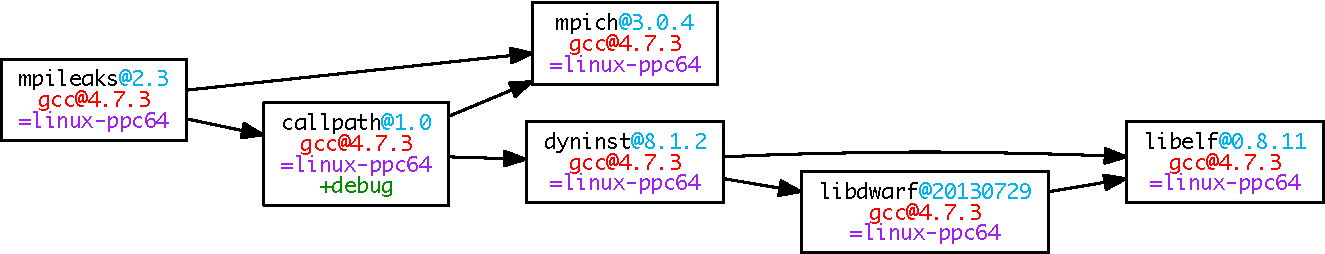
\includegraphics[width=\columnwidth]{specs/mpileaks-concrete.pdf}
	\caption{
		Concretized spec from Figure~\ref{fig:specs-mpileaks}.
		\label{fig:specs-mpileaks-concrete}
	}
\end{figure}
On completion, the concretization outputs a fully concrete spec DAG.
Figure~\ref{fig:specs-mpileaks-concrete} shows a concrete DAG with architectures,
compilers, versions, variants, and all dependencies resolved.
This fulfills Spack's guarantees.
%
At install time, Spack constructs a package object for each node in the spec DAG
and traverses the DAG in a bottom-up fashion.  At each node, it invokes the package's
{\tt install} method.  For the {\tt spec} parameter to {\tt install}, it passes
a sub-DAG rooted at current node (also a concrete spec).  Package authors must
query the spec in {\tt install} to handle different configurations.

\subsubsection{Concretization Runtime}
\label{sec:concretization-overhead}

\begin{figure}
	\centering
	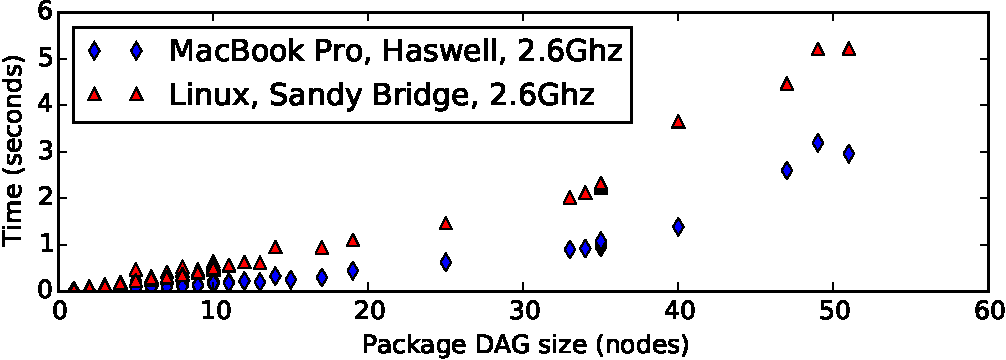
\includegraphics[width=.95\columnwidth]{figs/concretization-overhead/concretization-times.pdf}
	\caption{
		Concretization running time for 245 packages.
		\label{fig:concretization-time}
	}
\end{figure}

Figure~\ref{fig:concretization-time} shows the running time of concretization vs.
package DAG size in nodes.  We generated this plot by running {\tt concretize}
on all of Spack's 245 packages. We tested on three LLNL cluster front-end nodes:
a 2.3GHz Intel Haswell node and a 2.6 GHz Intel Sandy Bridge node on our Linux
clusters, and the 3.6 GHz IBM Power7 front-end node of a Blue Gene/Q system.
Each point is the average of 10 trials.  For all but the 10
largest packages, concretization takes less than 2 seconds on all machines.
For larger DAGs, we begin to see a quadratic trend, but even for 50 nodes or more,
concretization takes less than 4 seconds on the Haswell machine and 9 seconds on the
Power7.
%
We expect this performance from our greedy, fixed-point method, and
it is sufficient for the packages we have built so far.
Its running time is insignificant compared to the build time of
most packages, and it only executes
once per build.
More generally, concretization is an instance of the constraint
satisfaction problem, which is NP-complete. While concretization could become
more costly, we do not expect to see packages with
thousands of dependencies in the near future. We do not expect
it to become a bottleneck, even if we use a full constraint solver.

\subsubsection{Shared sub-DAGs}
\label{sec:directory-layout}

We mentioned in Section~\ref{sec:packages} that each unique configuration is
guaranteed a unique install prefix. Spack uses the concrete {\it spec}
to generate a unique path, shown in Table~\ref{tab:naming-conventions}.
To prevent the directory name from growing too long, Spack uses a SHA hash of
dependencies' specs as the last directory component.  However, Spack
does {\it not} rebuild every library for each new configuration.
If two configurations share a sub-DAG, then Spack reuses the sub-DAG's 
configuration.  Figure~\ref{fig:reuse} shows how the {\tt dyninst} sub-DAG 
is used for both the {\tt mpich} and {\tt openmpi} builds of {\tt mpileaks}.


\subsubsection{Reproducibility}


For reproducibility, and to preserve provenance, Spack stores a number of
files in the installation directory that document how the installed package was
built.  These include the {\tt package.py} file used to build, a build log
that contains output and error messages, and a file that contains the complete
concrete spec for the package {\it and} its dependencies. The spec file can be
used later to reproduce the build, even if concretization preferences have 
changed.

\subsubsection{Site policies and build complexity}

Our experience with manual installs helped us understand that much of the complexity
of building HPC software comes from the size of the build parameter space.
As previously mentioned, typical users only care about a few parameters.
The rest add unneeded complexity.  When building manually, LLNL staff
tend to make arbitrary choices about the secondary build parameters,
or they add logic to build scripts to make these choices.
Manually built software is generally not installed in a consistent manner.

Concretization provides two benefits.  First, it allows users and staff to
request builds with a minimal spec expression, while still providing a
mechanism for the site and the user to make consistent, repeatable choices 
for other build parameters.  For example, the site or the user can set 
default versions to use for any library that is not specified explicitly.
%
Second, concretization reduces the burden of packaging software, because
package authors do not have to make these decisions. Packages do not need 
to contain complicated checks, or to be overly specific about versions.  
Other multi-configuration systems like Nix, EasyBuild, and HashDist require 
the package author to write a mostly concrete build spec in advance.
This requirement puts undue burden on the package author, and it makes the task
of changing site policies within a software stack difficult.  Spack
separates these concerns.

\begin{figure}\centering
   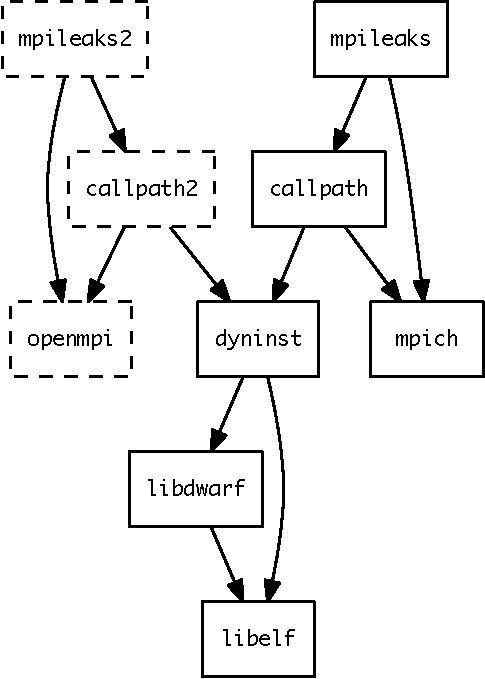
\includegraphics[width=.9\linewidth]{specs/rpaths.pdf}
   \caption{
       {\tt mpileaks} built with {\tt mpich}, then {\tt openmpi}.
       \label{fig:reuse}
   }
\end{figure}

%!TEX root = paper.tex


\subsection{Installation Environment}

%{\bf Reproducibility.}
%\paragraph{Reproducibility}
Spack is intended to build a consistent HPC stack for our multi-user
environment, and reproducible builds are one of our design goals.
Experience at LLNL has shown that it is vexingly difficult to reproduce
a build manually.
%
Many packages used at LLNL have a profusion of build options, and specifying them 
correctly often requires tedious experimentation.  This is due to lack of
build standards and to the diversity of HPC environments.  
For example, in some packages that depend on the {\tt Silo} library,
the \verb|--with-silo| parameter takes a path to {\tt Silo}'s installation prefix.
In others, it takes the {\tt include} and {\tt lib} subdirectories,
separated by a comma.
The {\tt install} method in Spack's package files allows us to record
precise build incantations for later reuse.

%{\bf Environment isolation.}
\paragraph{Environment isolation}
In addition to command-line issues, we
frequently encounter errors due to inconsistencies between the environment of
the package installer and the package user.
%
For example, there are two versions of the {\tt libelf} library used by
LLNL performance tools. One is distributed with RedHat Linux, while another
publicly available version has the same API but an incompatible ABI.
Failure to specify the right version at build time has caused many
unexpected crashes.
%
Spack manages the build environment by running each {\tt install} invocation
in a new process.  It helps packages find dependencies 
correctly, by setting
{\tt PATH}, {\tt PKG\_CONFIG\_PATH}, {\tt CMAKE\_PREFIX\_PATH}, and
{\tt LD\_LIBRARY\_PATH} to include the dependencies of the current build.
These variables are commonly used by build systems to locate dependencies,
and setting them helps to ensure that correct libraries are detected.
The isolated build environment also gives package authors 
free reign to set build-specific environment variables without interfering
with other packages.


%{\bf Compiler wrappers and RPATHs.}
\paragraph{Compiler wrappers and RPATHs}
Finding compilers at build time is not the only obstacle to reproducible
behavior.  As mentioned in Section~\ref{sec:motivation}, it is also important
for binaries to be able to find dependency libraries at {\it runtime}.
One of the most frequent user errors at LC is improper library configuration.
Users frequently do not know what libraries a package was built with, and 
it is difficult for them to construct a suitable {\tt LD\_LIBRARY\_PATH} for
a package that was built by someone else.  Because of frequent support calls,
we typically add {\tt RPATHs} to public software installations, so that paths
to dependencies are embedded in binaries and so that users do not have to know
this information to run installed software correctly.

Spack manages {\tt RPATH} settings and other build policies with
{\it compiler wrappers}. 
In each isolated {\tt install} environment, Spack sets the standard 
environment variables
{\tt CC}, {\tt CXX}, {\tt F77}, and {\tt FC} to point to its own compiler
wrapper scripts.  These variables are used by most build systems to select
C, C++, and Fortran compilers, so they are generally picked up 
automatically\footnote{If builds do not respect {\tt CC}, {\tt CXX}, etc.,
wrappers can be added as arguments or inserted into Makefiles
by {\tt install}.}.
When run, the wrappers insert include ({\tt -I}), library ({\tt -L}), and 
{\tt RPATH} ({\tt -Wl,-rpath} or similar) flags into the argument list.
These point to the {\tt include} and {\tt lib} directories of dependency
library installations, where needed headers and libraries are located.
The wrappers then invoke the real compiler with the modified arguments.

Spack's compiler wrappers have a number of useful effects.  First, they allow
Spack to transparently switch compilers in most builds.  This is how
compiler options like {\tt \%gcc} are implemented.  Second, they enforce the
use of {\tt RPATHs} in
installed binaries.  This causes applications built by Spack to run correctly
{\it regardless of the environment}.  Third, because compiler wrappers add 
header and library search paths for dependencies, header and library detection
tests run by most build systems succeed automatically, {\it without}
the need to use special arguments for nonstandard locations.  {\tt configure}
commands in Spack's {\tt install} function can have fewer arguments, and can
be written as they would be for system installs.  This reduces complexity
for package maintainers and enforces consistent, reproducible
build policies across packages.  Finally, because Spack has control over the 
wrappers, package authors can programmatically filter the compiler flags
used by software build systems, a useful last resort when porting to
bleeding-edge platforms or new, esoteric compilers.

\subsubsection{Environment Module Integration}
\label{sec:envmodule}
In addition to managing the build-time environment, Spack can assist in managing
the run-time environment.  A package may need environment variables like {\tt PATH}, 
{\tt LD_LIBRARY_PATH}, or {\tt MANPATH} set before they can be used.  
As discussed in Section~\ref{sec:motivation}, many sites rely on environment 
modules to set up the runtime environment.  Spack can automatically create simple
dotkit~\cite{dotkit} and Module configuration files for its packages, allowing 
users to setup their runtime environment using familiar systems.  
%
Future versions of Spack may also allow the creation of Lmod~\cite{mclay:lmod} 
hierarchies, as discussed in Section~\ref{sec:env-rpath}. Spack's rich 
dependency information would allow such hierarchies to be generated automatically.

















%!TEX root = paper.tex

\section{Use Cases}
\label{sec:usecases}


%!TEX root = paper.tex

\subsection{Combinatoric Names}
\label{sec:usecase-combinatoric}


\subsubsection{Gperftools packaging}

The gperftools tool from Google has gained popularity among some developers for
its high-performance thread-safe heap and its lite-weight profilers.  
Unfortunately, two issues made it difficult to maintain gperftools installations 
at LLNL.  First, gperftools is a C++ library.  Since C++ does not have standard 
ABI it needs to be re-built with each compiler and compiler version.  Second, 
building gperftools on atypical architectures (such as Blue Gene/Q) requires 
patches and a complicated configure lines that change with each compiler.  The 
first issue motivated application developers to try and maintain their own builds 
of gperftools that worked with their prefered compilers--a task that was made 
difficult by the second issue.

Spack presented a solution to both problems.  Package administrators can use Spack to 
easily maintain a central install of gperftools across the combinations of versions 
and compilers.  Spack's gperftools package also serves as a central repository for 
the knowledge of how to build gperftools on each platform and compiler combination.  

\begin{figure}
  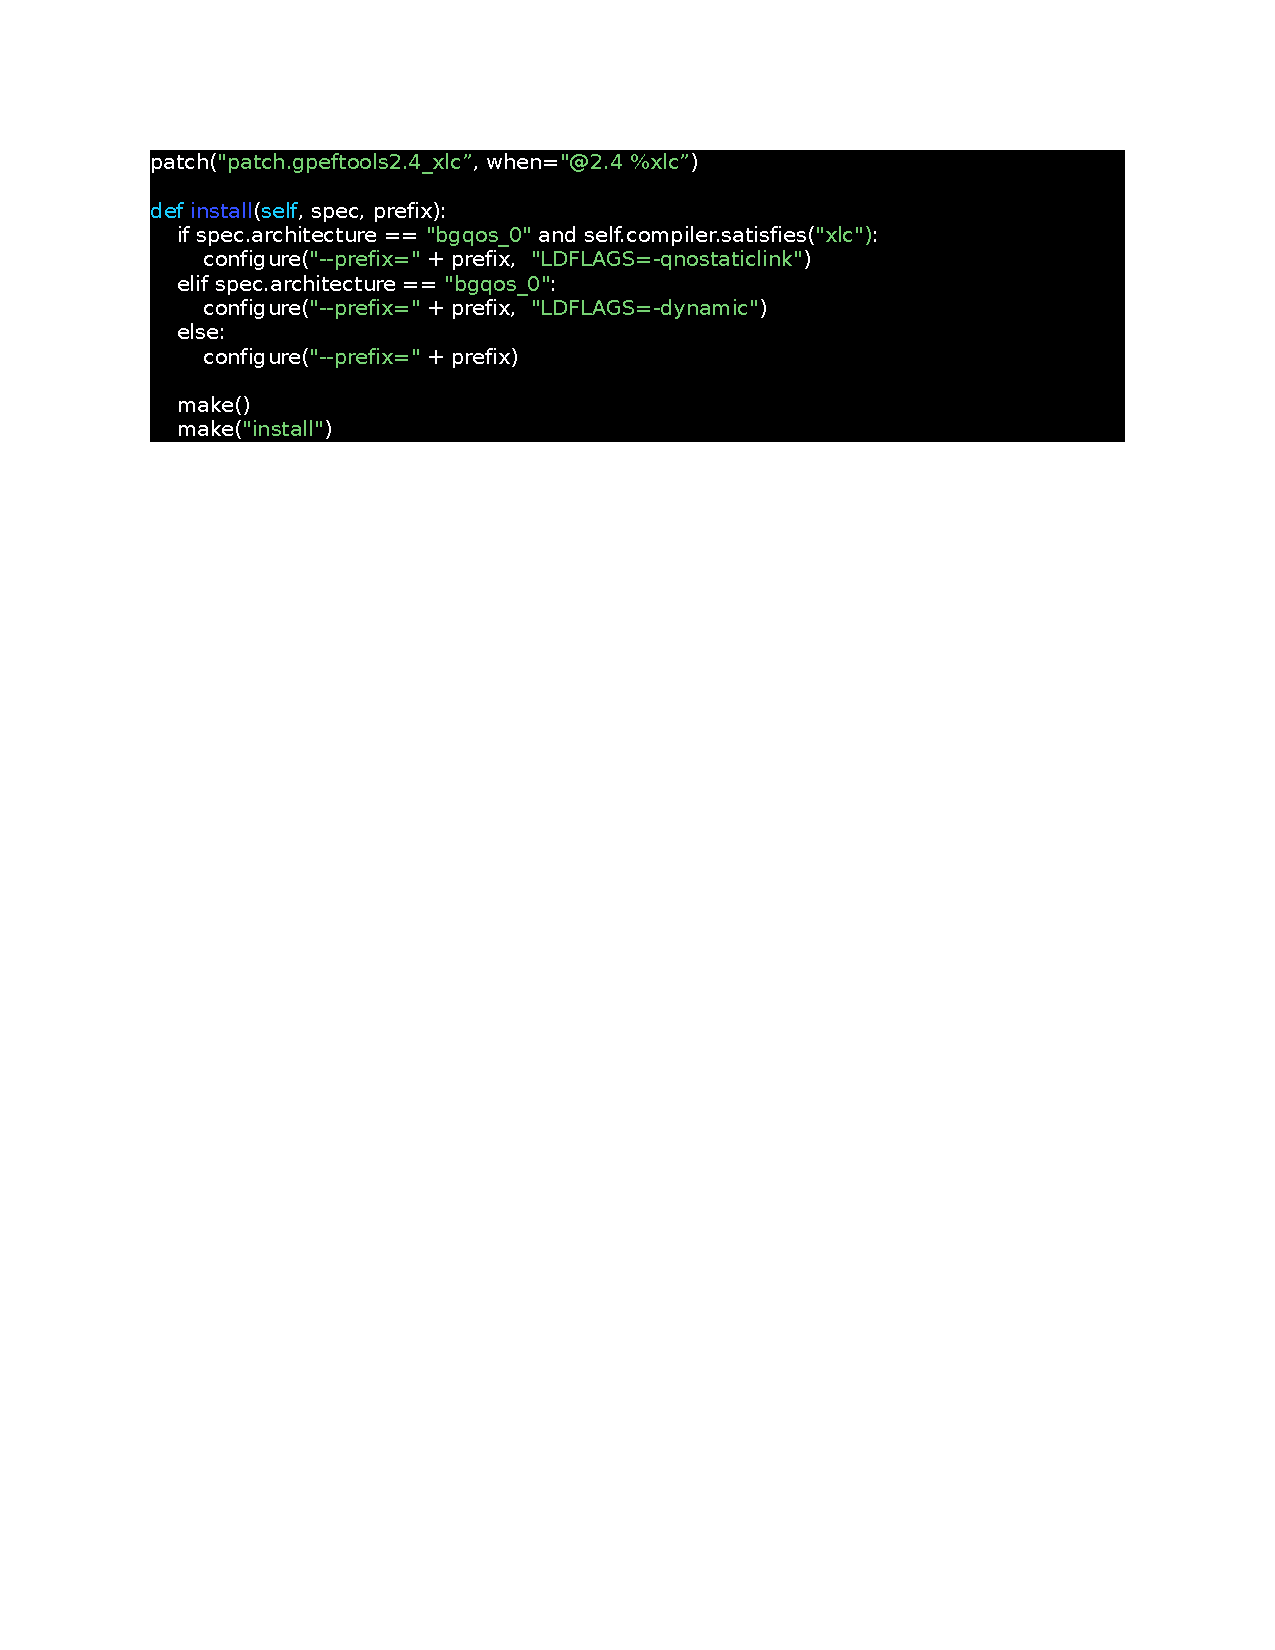
\includegraphics[width=\columnwidth]{code/gperftools.pdf}
  \caption{
    Simplified install routine for the gperftools tool.
    \label{fig:gperftools}
  }
\end{figure}

Figure~\ref{fig:gperftools} illustrates per-compiler and platform build rules with 
a simplified version of the install routine for the gperftools tool (Spack's real 
install routine for gperftools includes other compilers and more options per
compiler).  It applies a patch if gperftools 2.4 is built with the XLC compiler, 
and it selects the correct configure line based on the current platform and compiler.  

\subsubsection{{\tt mpileaks} packaging}
\todo{.5 page}
\begin{verbatim}
	- compiler x version x MPI x mpi version
\end{verbatim}


%!TEX root = spack-sc15.tex

\subsection{Support for interpreted languages}
\label{sec:usecase-python}

Python is becoming increasingly popular for HPC applications,
due to its flexibility as a language and its excellent support
for calling into fast, compiled numerical libraries.
Python is an interpreted language, but one can use it
as a friendlier interface to compiled libraries like FFTW, ATLAS, and
other linear algebra libraries.  Many LLNL code teams use Python in this manner.
%
LC supports Python installations for several application teams,
and maintaining these repositories has grown increasingly complex over
time. The problems are similar to those that drove us to create
Spack: different teams want different Python libraries with different
configurations.

Existing Python package managers are either language-specific~\cite{eby:setuptools},
or they do not support building from source~\cite{anaconda,conda}. None
handles multi-configuration builds.  More glaringly, Python extensions
are usually installed into the Python interpreter's prefix.
This makes it impossible to install multiple versions.\footnote{{\tt setuptools}
has support for multiple versions via {\tt pkg_resources},
but this requires modifications to client code.}
Installing each extension in its own prefix enables combinatorial versioning,
but it requires users to add packages to the {\tt PYTHONPATH} variable at runtime.

Per Spack's design philosophy, we wanted a way to easily manage many different
versions, but {\it also} to provide a baseline set of extensions {\it without}
requiring environment settings.
%
To support this mode of operation, we added the concept of {\tt extension} packages
to Spack. Python modules use the {\tt extends('python')} directive instead of
{\tt depends\_on('python')}.
Each module installs into its own prefix like any other package,
and each module depends on a particular Python installation.
But extensions can be {\tt activated} or {\tt deactivated} an
within the dependent Python installation.  The {\tt activate} operation
symbolically links each file in the extension prefix into the Python
installation prefix, as though it were installed directly. If any file
conflict would arise from this operation, {\tt activate} fails.
Similarly, the {\tt deactivate} operation removes the symbolic links and restores
the Python installation to its  pristine state.

There were additional complications because many Python packages {\it install their own
package manager} if they do not find one in the Python installation.
There are also many ways that Python packages add themselves to the
interpreter's default path, and some of them conflict. We modified
Spack so that extendable packages, like Python, can supply custom code
in the package file that that specializes {\tt activate} and {\tt deactivate}
for the particular package. Python uses this feature to merge conflicting
files during activation.  The end result is that Python extensions can
be installed automatically in their own prefixes, and they can be composed
with a wide range of bleeding-edge libraries that other package managers do
not handle.

%To experiment with these extensions, users can load environment
%modules generated by Spack. If they want a particular version to be available
%without any special environment settings, they can activate it within the Python instance.

Spack essentially implements a ``meta package-manager'' for each Python
instance, which can coexist with Spack's normal installation model.
This has allowed us to efficiently support our application teams, for whom we can
now rapidly construct custom Python installations.  We have also reduced
the amount of time that LC staff spend installing Python modules.
Because Spack packages can extend the activation and deactivation mechanisms,
we believe the same mechanism could be used with other
interpreted languages with similar extension models, such as R, Ruby, or Lua.

%!TEX root = paper.tex

\subsection{User and Site Policies}
\label{sec:usecase-policy}

Spack makes it easy for package maintainers to create and organize package installations.  But it also needs to be easy for end-users to find and use those packages.  Different end-users may have different expectations about how packages should be built and installed, and those expectations are typically shaped by years of site policies, personal preferences, and lingering legacy decisions originallly made on a DEC VAX.  Rather than try to dictate these expectations, Spack allows both end-users and package maintainers to create custom policies dictating how packages are built and installed at their site.

\subsection{Package Views}
\label{sec:package-views}

While Spack can easily create a dozen installations of a package like {\tt mpileaks} for different compilers and MPI implementations, it can be difficult for an end-user to determine which of those dozen packages should be used with their application.  As discussed in Section~\ref{sec:envmodule}, environment modules are commonly used on supercomputer systems to solve this problem, and Spack allows the package administrator to automatically create module and dotkit files for packages that Spack installs.

However, even when modules and dotkits are available, many users will go directly through the filesystem to access package installs.  Spack installs packages into paths based on concretized specs, which is ideal for maintaining multiple package installations, but may be difficult for an end-user to navigate.  A version of {\tt mpileaks}, for example, may be installed in a location like:
%
\begin{minted}[fontsize=\scriptsize]{bash}
    spack/opt/chaos_5_x86_64_ib/gcc@4.9.2/mpileaks@1.0-db465029
\end{minted}
%
Spack thus allows the creation of views, which are a symbolic-link based directory layout of packages.  Views provide a human-readable directory layout, which can be tailored to fit alongside existing directory layouts or used to create new layouts.  For example, the above {\tt mpileaks} package may have a view that creates a link in {\tt /opt/mpileaks-1.0-openmpi} to the Spack installation of {\tt mpilleaks}.  The same package install may be referenced by multiple links and views, so the above package could also be linked from a more generic {\tt /opt/mpileaks-openmpi} link (which is useful for users who don't want to hardcode a specific version).  Views can also be used to create links to specific executables or libraries in an install, so a Spack-built {\tt gcc 4.9.2} install may have a view that creates links from {\tt /bin/gcc49} and {\tt /bin/g++49} to the appropriate {\tt gcc} and {\tt g++} executables.

Views are configured through a {\tt spackconfig} file, which can be setup at a site-wide level or for individual users.  For each package or set of packages, the {\tt spackconfig} file contains rules describing the links that should point into that package.  The link names can be parameterized.  For example, the above {\tt mpileaks} link might have been created by rule like:
%
\begin{minted}[fontsize=\scriptsize]{bash}
    /opt/${PACKAGE}-${VERSION}-${MPINAME}
\end{minted}
%
When Spack installs or removes packages, symbolic links are automaticaly created, deleted, or updated according to these rules.  

Spack's views are a projection from a point in a high-dimensional space (the directory layout shown in Table~\ref{tab:naming-conventions}, which fully specifies all parameters) to point in a lower-dimension space (the link name, which may only specify a few parameters).  Thus several package installations may map to the same symbolic link.  For example, the above {\tt mpileaks} link could point to an {\tt mpileaks} compiled with {\tt gcc} or {\tt icc} -- the compiler parameter is not part of the link.  To keep  package installations  consistent and reproducible, Spack has a well-defined mechanism for resolving conflicting links.  Spack defines a sort order for packages, which arranges packages from ``most desired'' to ``least desired''.  When a symlink could resolve to multiple package installations, Spack points the symlink at the most desired package.  

By default, Spack treats newer versions of packages compiled with newer compilers as more desirable than older packages built with older compilers.  It has well-defined, but not necessarily meaningful, preferences for deciding between MPI implementations and different compilers.  A user can override Spack's default sort order through their {\tt spackconfig} file.  For example, at one site users may typically use the Intel compiler, but some users also use the system's default {\tt gcc 4.4.7}.  These preferences could be stated by adding the line:
%
\begin{minted}[fontsize=\scriptsize]{bash}
    compiler_order = icc,gcc@4.4.7
\end{minted}
%
to the site's {\tt spackconfig} file, which would cause the ambigious {\tt mpileaks} symlink to point to an {\tt icc} installation.  Any compiler left out of the {\tt compiler\_order} setting is treated as less preferred than those explicitly mentioned.  Spack also supports allowing specific package versions and other spec options as more preferred than others.  This is useful for deploying unstable or untested software within Spack before moving it into wider public view.  


\subsection{Site-specific Package Repositories}

By default, Spack stores its package files in a mainline repository that is present when users
first run Spack.  At many sites, packages may build sensitive, proprietary software, or they 
may have patches that are not useful outside of a certain company or organization.  Putting
this type of code back into a public repository does not often make sense, and if it makes the
mainline less stable, it can actually make sharing code between sites more difficult.  

To support our own private packages, and to support those of LLNL code teams, Spack allows he creation of site-specific variants of packages.  

The build instructions for a Spack package are encoded in a Python class, which must inherit from Spack's {\tt Package} class.  Via the {\tt spackconfig} file, users can specify additional search directories for finding additional {\tt Package} classes.  These additional packages can inherit from and replace the Spack's default packages, allowing sites to either tweak or completely replace Spack's build recipes.  To continue the previous example, a site can write a {\tt LocalSpindle} Python class, which inherits from Spack's {\tt Spindle} class.  {\tt LocalSpindle} may simply add additional configure flags to the {\tt Spindle} class, while leaving the dependencies and most of the build instructions from its parent class.  To keep builds deterministic and reproducable, Spack also tracks which {\tt Package} class drove a specific build. 










%!TEX root = spack-sc15.tex

\section{Conclusion}
\label{sec:conclusion}


The complexity of managing HPC software is rapidly increasing, and it
will continue unabated without better tools.
In this paper, we reviewed the state of software management tools
across a number of HPC sites, with particular focus on Livermore
Computing (LC). While tools exist that can handle multi-configuration
installs, none of them addresses the combinatorial nature
of the software configuration space directly. None of them allows
a user to rapidly {\it compose} new parametric builds.

We introduced Spack, a package manager in development at LLNL, that
provides truly {\it parameterized} builds.  Spack implements
a novel, recursive {\it spec} syntax that simplifies the process of working
with large software configuration spaces, and it builds software
so that it will run correctly, regardless of the environment.
We outlined a number of Spack's unique features, including
versioned virtual dependencies, and the {\it concretization} process,
which converts an underspecified build DAG into a buildable spec.

We showed through three use cases that Spack is already
increasing operational efficiency
in production at LLNL.  We believe that the software management
techniques implemented in
Spack are applicable to a broad range of HPC facilities.
Spack is available online at: http://bit.ly/spack-git.


%\raggedright
%\footnotesize
\bibliographystyle{abbrv}
\bibliography{paper}

\end{document}
